\section{LIMDD}


\begin{frame}[noframenumbering]
\begin{refsection}

\vfill
	
	\centering
	\textbf{\Large Decision Diagrams in Quantum Circuit Compilation}
	
	
\vfill

\printbibliography[section=\therefsection]
\end{refsection}

\end{frame}







%\begin{refframe}{Decision Diagrams for Representing Pseudo-Boolean Functions}
%	
%\vspace{-.8em}
%
%
%%\begin{block}{History of DDs for representing a function $\set{0,1}^n\to \complex$}
%\begin{itemize}
%	\item<+->[(1993)] Multi-Terminal DD (MTBDD)~\cite{clarke1993spectral}
%
%\vspace{-1em}\hfill
%\tikzset{every picture/.style={->,thick}}
%~\hspace{-1cm}
%\begin{tikzpicture}[
%    scale=0.3,
%    every path/.style={>=latex},
%    every node/.style={},
%    inner sep=0pt,
%    minimum size=0.3cm,
%    line width=1pt,
%    node distance=1cm,
%    thick,
%    font=\footnotesize
%    ]   
%
%
%    % nodes
%    \node[draw,circle] (a1) {$x_1$};
%    \node[draw,circle, below = .45cm of a1, xshift=-.4cm] (a2) {$x_2$};
%    \node[draw,circle, below = .45cm of a1, xshift= .4cm] (a3) {$x_2$};
%%    \node[draw,circle, below = .45cm of a2, xshift=-.3cm] (a41) {};
%    \node[leaf,below = .45cm of a2, xshift=-.3cm] (a42) {$2$};
%    \node[leaf,below = .45cm of a3, xshift=-.4cm] (a43) {$1$};
%    \node[leaf,below = .45cm of a3, xshift= .3cm] (a44) {$-2$};
%
%    \draw[e0 = 0] (a1) edge  node[] {} (a2);
%    \draw[e1 = 0] (a1) edge  node[] {} (a3);
%
%    \draw[e0=  0] (a2) edge  node[] {} (a43);
%    \draw[e1=  0] (a2) edge  node[] {} (a42);
%    \draw[e0=  0] (a3) edge  node[] {} (a43);
%    \draw[e1=  0] (a3) edge  node[] {} (a44);
%\end{tikzpicture}
%%	\item[(1997)] Algebraic DD (ADD)~\cite{bahar1997algebric}   \hfill = MTBDD
%\vspace{1ex}
%
%
%	\item<+->[(1994)] Edge-Valued DD (EVDD)~\cite{lai1994evbdd} 
%	
%\vspace{-1em}\hfill
%\tikzset{every picture/.style={->,thick}}
%~\hspace{-1cm}
%\begin{tikzpicture}[
%    scale=0.3,
%    every path/.style={>=latex},
%    every node/.style={},
%    inner sep=0pt,
%    minimum size=0.3cm,
%    line width=1pt,
%    node distance=1cm,
%    thick,
%    font=\footnotesize
%    ]   
%
%
%    % nodes
%    \node[draw,circle] (a1) {$x_1$};
%    \node[draw,circle, below = .45cm of a1, xshift=-.7cm] (a2) {$x_2$};
%    \node[draw,circle, below = .45cm of a1, xshift= .7cm] (a3) {$x_2$};
%    \node[leaf, below = .45cm of a2, xshift= .7cm] (a41) {$1$};
%    
%    % edges
%    \draw[e0 = 0] (a1) edge  node[] {} (a2);
%    \draw[e1 = 0] (a1) edge  node[] {} (a3);
%
%    \draw[e0= 20] (a2) edge  node[left,pos=.4] {} (a41);
%    \draw[e1= 20] (a2) edge  node[above right,pos=.3] {~$2$} (a41);
%    \draw[e0= 20] (a3) edge  node[left,pos=.] {} (a41);
%    \draw[e1= 20] (a3) edge  node[right,pos=.4] {$-2$} (a41);
%\end{tikzpicture}
%\vspace{1ex}
%
%
%%	\item[(2005)] Semiring-labeled DD (SLDD)~\cite{wilson2005decision} \hfill = EVDD
%%	\item[(1997)] Factored edge-Valued DD (FEVDD)~\cite{tafertshofer1997factored}
%%	\item[(2005)] Affine Algebraic Decision Diagram (AADD)~\cite{aadd}  \hfill = FEVDD
%	\item<+->[(2011)] Sentential DD (SDD)~\cite{kisa2014probabilistic}
%
%
%\vspace{-1em}\hfill
%\tikzset{every picture/.style={->,thick}}
%\hspace{-1cm}
%\begin{tikzpicture}[
%    scale=0.3,
%    every path/.style={>=latex},
%    every node/.style={},
%    inner sep=0pt,
%    minimum size=0.3cm,
%    line width=1pt,
%    node distance=1cm,
%    thick,
%    font=\footnotesize
%    ]   
%
%
%    % nodes
%    \node[draw,circle] (a1) {};
%    \node[draw,circle, below = .45cm of a1, xshift=-.7cm] (a2) {};
%    \node[draw,circle, below = .45cm of a1, xshift= .7cm] (a3) {};
%    
%    % edges
%    \draw[e0 = 0] (a1) edge  node[above left] {$x_1\lor x_2$} (a2);
%    \draw[e1 = 0] (a1) edge  node[above right] {$\overline x_1 \land \overline{x_2}$} (a3);
%\end{tikzpicture}
%\end{itemize}
%\vspace{-1em}
%
%%\end{block}
%
%\end{refframe}












\begin{refframe}[fragile]{Quantum State Representation with
					\alert{Decision Diagrams}}

%\vspace{-1em}
We can think of a quantum state $\vec v$ as a pseudo Boolean function $f \colon \set{0,1}^n \to \complex$, or alternatively as an exponentially-sized complex vector:

~\\
\pause

\centering

\tikzset{every picture/.style={->,thick}}
~\hspace{-1cm}
\begin{tikzpicture}[
    scale=0.3,
    every path/.style={>=latex},
    every node/.style={},
    inner sep=0pt,
    minimum size=0.3cm,
    line width=1pt,
    node distance=1cm,
    thick,
    font=\footnotesize
    ]


    % nodes
    \node[draw,circle] (a1) {};
    \node[draw,circle, below = .45cm of a1, xshift=-.9cm] (a2) {};
    \node[draw,circle, below = .45cm of a1, xshift= .9cm] (a3) {};
%    \node[draw,circle, below = .45cm of a2, xshift=-.3cm] (a41) {};
    \node[draw,circle, below = .45cm of a2, xshift= .3cm] (a42) {};
    \node[draw,circle, below = .45cm of a3, xshift=-.3cm] (a43) {};
    \node[draw,circle, below = .45cm of a3, xshift= .3cm] (a44) {};

%\only<-2,5->{
    \node[leaf, below= .45cm of a42, xshift= -.13cm, inner sep=0pt] (w3) {$2$};
    \node[leaf, right= .32cm of w3,inner sep=0pt] (w5) {$1$};
    \node[leaf, right= .32cm of w5,inner sep=0pt] (w7) {$-2$};

    \draw[e0= 0] (a42) edge   (w3);
    \draw[e0= 0] (a43) edge   (w5);
    \draw[e0= 0] (a44) edge  (w7);
%}

%\only<3-4>{
%    \node[leaf, below= .45cm of a42, xshift=.6cm] (w1) {$1$};
%    
%    \draw[e0= 0] (a42) edge  node[above right,pos=.3] {$2$} (w1);
%    \draw[e0= 0] (a43) edge  node[above left,pos=.3] {} (w1);
%    \draw[e0=-20] (a44) edge  node[pos=.4,below right] {$-2$} (w1);
%}


    % edges
    \draw[<-] (a1) --++(90:2cm) node[right,pos=.7] {};
    \draw[e0 = 0] (a1) edge  node[] {} (a2);
    \draw[e1 = 0] (a1) edge  node[] {} (a3);

    \draw[e0=  0] (a2) edge  node[] {} (a43);
    \draw[e1=  0] (a2) edge  node[] {} (a42);
    \draw[e0=  0] (a3) edge  node[] {} (a43);
    \draw[e1=  0] (a3) edge  node[] {} (a44);

  
\node[left = 1.3cm of a1.south,yshift=-1cm] (vec) {
    \begin{minipage}{1.7cm}\footnotesize
    $
%\frac 12\cdot
\def\arraystretch{1.3}
    \begin{bmatrix*}[r]
			 \only<4->{\color{red} 1}\only<-3>{1}\\\only<4->{\color{red} 0}\only<-3>{0}\\
    		 \only<7->{\color{purple} 2}\only<-6>{2}\\\only<7->{\color{purple} 0}\only<-6>{0}\\
    		\only<4->{\color{green} 1}\only<-3>{1}\\\only<4->{\color{green} 0}\only<-3>{0}\\ 
    		\only<7->{\color{blue}-2}\only<-6>{-2}\\
    		\only<7->{\color{blue} 0}\only<-6>{0} \\
    \end{bmatrix*}$
    \end{minipage}
};


 \node[below= 2.5cm of a1,text width= 2.99cm]  (add)   {\centering Multi-Terminal DD (MTBDD)};

\pause[3]

%    \node[draw,circle, below = .45cm of a2, xshift=-.3cm,fill=red] (a41) {};
    \node[draw,circle, below = .45cm of a2, xshift= .3cm,fill=purple] (a42) {};
    \node[draw,circle, below = .45cm of a3, xshift=-.3cm,fill=green] (a43) {};
    \node[draw,circle, below = .45cm of a3, xshift= .3cm,fill=blue] (a44) {};

\only<3>{
\node[right= of a3, text width = 3cm] {
\color{green}$f_{00} = f_{10} = \begin{bmatrix*}[c]
    				   1, \\ 0\phantom{,}\\
    				\end{bmatrix*}$\\\vspace{4mm}
\color{purple}\scriptsize$f_{01}  =\phantom-2\cdot  f_{00}$\\\vspace{4mm}
%\color{green}\scriptsize$ f_{10} = \phantom-2\cdot  f_{00}$\\\vspace{4mm}
\color{blue}\scriptsize$f_{11}=-2 \cdot f_{00}$
};
}


\pause


    % nodes
    \node[draw,circle, right= 2.8cm of a1] (a1) {};
    \node[draw,circle, below = .45cm of a1, xshift=-.7cm] (a2) {};
    \node[draw,circle, below = .45cm of a1, xshift= .7cm] (a3) {};
    \node[draw,circle, below = .45cm of a2, xshift= .7cm,shade, shading=axis, left color=purple,  middle color=purple, right color=blue, shading angle=90] (a41) {};
    \node[leaf, below= .45cm of a41] (w1) {$1$};

    
    % edges
    \draw[<-] (a1) --++(90:2cm) node[right,pos=.7] {};
    \draw[e0 = 0] (a1) edge  node[] {} (a2);
    \draw[e1 = 0] (a1) edge  node[] {} (a3);

    \draw[e0= 20] (a2) edge  node[left,pos=.4] {} (a41);
    \draw[e1= 20] (a2) edge  node[above right,pos=.3] {~$2$} (a41);
    \draw[e0= 20] (a3) edge  node[left,pos=.] {} (a41);
    \draw[e1= 20] (a3) edge  node[right,pos=.4] {$-2$} (a41);
    \draw[e0=0] (a41) edge  node[left] {} (w1);
%    \draw[e1=25] (a41) edge  node[lbl,right] {$0$} (w1);

\node[below= 2.5cm of a1,text width= 2.6cm] (aadd) {\centering Edge-Valued DD (EVDD)};


\pause

\node[below= .3cm of add, xshift=-2cm] {\alert{\textbf{Merge nodes $v, w$: }}};
\node[below= .3cm of add] {\alert{$\vec v = \vec w$ }};
\node[below= .3cm of aadd, xshift=.cm,text width = 4cm,align=center] {\alert{$\vec v = \gamma \cdot \vec w$\\ \vspace{3mm}(equivalent up to a complex factor $\lambda$)}};

    \onslide<1->
\end{tikzpicture}

\onslide<+->{
\centering
\alert{(EVDD can be exponentially more succinct than MTBDD.)}
}


\phantom{
\cite{fujita1997multi,Vrudhula1996}
}


\end{refframe}




%\begin{refframe}{Chronology of Decision Diagrams for Pseudo-Boolean Functions}
%	
%\vspace{-.8em}
%
%
%\begin{table}
%\centering\footnotesize
%\def\arraystretch{1.4}
%\begin{tabular}{|p{5.5cm}|c|c|}
%\hline
%\textbf{Decision diagrams for pseudo-Boolean functions}				& \textbf{Node merging strategy} &  \\\hline
%%Decision Tree	& (no merging) &  \\
%MTBDD~(1993)~\cite{clarke1993spectral}, \add~(1997)~\cite{bahar1997algebric}	& $f = g$  &  \\
%SLDD$_\times$~(2005)~\cite{wilson2005decision}	& $f = \gamma\cdot g$   & $\gamma \in \complex, \mathbb R, \dots$  \\
%EVBDD (1994)~\cite{lai1994evbdd}, SLDD$_+$ (2013)~\cite{fargier2013semiring}	& $f = g + \alpha$ & $\alpha \in \complex, \mathbb R, \dots$  \\
%FEVBDD~(1997)~\cite{tafertshofer1997factored}, AADD~(2005)~\cite{aadd}		& $f = \gamma\cdot g + \alpha$ & $\alpha,\gamma \in \complex, \mathbb R, \dots$ \\
%%\limdd~\cite{limdd}			& $f = \gamma  P_1\otimes \dots \otimes P_n \cdot g$ & $P_i \in \gen{\id, X,Y,Z}$   \\
%\hline
%\end{tabular}
%\end{table}
%
%\vspace{-.8em}
%
%
%%\nocite{limdd2}
%
%\end{refframe}




%\begin{refframe}{Chronology of Decision Diagrams in Quantum Computing}
%	
%\vspace{-.8em}
%
%	
%\begin{table}
%\centering\footnotesize
%\def\arraystretch{1.5}
%\begin{tabular}{|p{4.5cm}|p{1.5cm}|c|c|}
%\hline
%\textbf{Quantum variant}	&
%\textbf{Original}				& \textbf{Node merging} &  \\\hline
%%Decision Tree	& (no merging) &  \\
% QuiDD~(2003)~\cite{viamontes2003improving}					    &MTBDD (1993)  & $f = g$  &  \\
% QMDD~(2006)~\cite{qmdd}, Tensor DD~(2020)~\cite{hong2022tensor}   & EVDD~(1994)  &$f = \gamma\cdot g$   & $\gamma \in \complex, \dots$  \\
%%SLDD$_+$~\cite{fargier2013semiring}, EVBDD~\cite{lai1994evbdd}	& $f = g + \alpha$ & $\alpha \in \complex, \mathbb R, \dots$  \\
%%AADD~\cite{sanner2005AffineADDs}, FEVBDD~\cite{tafertshofer1997factored} 		& $f = \gamma\cdot g + \alpha$ & $\alpha,\gamma \in \complex, \mathbb R, \dots$ \\
%%&\limdd~(2021)~\cite{limdd}			& $f = \gamma  P_1\otimes \dots \otimes P_n \cdot g$ & $P_i \in \gen{\id, X,Y,Z}$   \\
%%%&QDD~(TODO)~\cite{TODO}					& () \\
%%&CFLOBDD~(2023)~\cite{TODO}				& (more like SDD)  \\
%\hline
%\end{tabular}
%\end{table}
%
%\vspace{-.3em}
%
%
%
%\begin{block}<2->{Applications for Quantum Circuits:}
%\begin{itemize}
%	\item Simulation			\hfill   $G_k\cdots G_1 \cdot \vec v$
%	\item Equivalence checking	 \hfill $U \cdot V^\dagger = I$
%%	\item Synthesis / optimization~\cite{abdollahi2006analysis,amy2013meet,zulehner2017improving}
%\end{itemize}
%\end{block}
%
%
%\begin{alertblock}<3->{Exploiting Historical Parallels}
%	\begin{itemize}
%	\item<+-> Addition is hard for EVDD~\cite{fargier2013semiring}, hence Hadamard gates are hard for QMDD
%	\item<+-> EVDD is prone to numerical instability (\cite{aadd}), and so is QMDD~\cite{niemann2020overcoming}
%	\end{itemize}
%\end{alertblock}
%\vspace{-.8em}
%
%
%\end{refframe}




\begin{refframe}{Performance of DD-based methods}
\centering

	~~~~~~~~QFT~~~~~~~~~~~~~~~~~~~~~~~~~~~Shor~~~~~~~~~~~~~~~~~~~~~~~~~~~~Grover\vspace{-1em}

	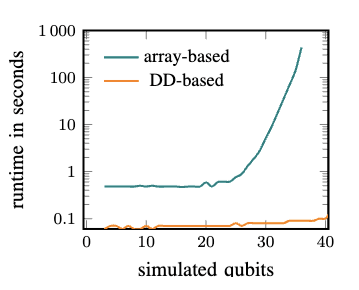
\includegraphics[height=3.2cm]{graphics/perf-qft}\hspace{-1em}
	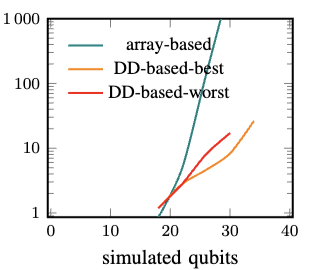
\includegraphics[height=3.1cm]{graphics/perf-shor}\hspace{-1ex}	
	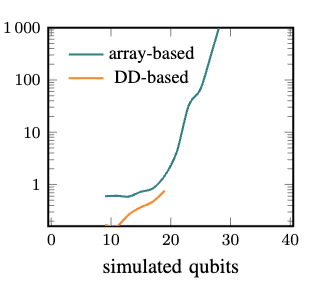
\includegraphics[height=3.1cm]{graphics/perf-grover}

\begin{alertblock}{Performance Characteristics for Simulation~\cite{grurl2020arrays}}
	\begin{itemize}
		\item Very fast and memory-efficient for structured quantum circuits
		\item EVDD is prone to numerical instability~\cite{niemann2020overcoming}; exact representations solve this~\cite{9586191} 
	\end{itemize}
\end{alertblock}

\vspace{-1em}

\end{refframe}













%\end{comment}









\begin{refframe}{Analysis of Quantum Decision Diagrams}

\centering
\begin{tikzpicture}\footnotesize
  \tikzset{venn circle/.style={circle,minimum width=2cm,fill=####1,opacity=0.4}}
  \node [venn circle=white,minimum width=2.5cm,draw] (A) at (0,0.3) {};
  \node  at (0,1.25) 			{Quantum states};

%  \node [venn circle = Red!40!white, ellipse,minimum height=2.2cm, minimum width=3.6cm] (L) at (0,0.6) {};
%  \node  at (0,1.5) 		{\limdd};
  
%  \node [venn circle = blue!70!white,text width=1.3cm,align=center,rotate=79,ellipse,minimum height=1.8cm, minimum width=2.5cm] (B) at (-.6,-.2) {};
%  \node[text width=1.3cm,align=center]  at (-.9,-1.) {MPS};


%  \node [venn circle = green!70!white,text width=1.3cm,align=center,rotate=119,ellipse,minimum height=1.8cm, minimum width=2.5cm] (B) at (.6,-.2) {};
%  \node[text width=1.3cm,align=center]  at (.9,-1.) {RBM};



%  \node [venn circle = Blue!100!white,text width=1cm,align=center, minimum width=1.cm] (B) at (-.5,.3) 	{\textcolor{white}{QMDD}};						

  \node [venn circle = OliveGreen,text width=1cm,align=center, minimum width=.8cm,opacity=.5,text opacity=1] (C) at (.5,.2) {\textcolor{white}{Stabilizer states}};
\end{tikzpicture}	

\alert{Stabilizer circuits are non-universal \& classically simulatable, but crucial in error correction, etc.}

\pause


\begin{alertblock}{EVDD can't succinctly represent stabilizer states, yet:}
	\begin{itemize}
%		\item For \alert{stabilizer states}, we proved  that EVDD can be exponential
		\item Stabilizers are a subset of states that are \alert{classically simulatable!}
		\item Important in error correction, measurement-based QC and circuit equivalence
	\end{itemize}
\end{alertblock}


\begin{theorem}[\cite{limdd} ]
EVDD requires $2^{\Omega({{n}})}$ space to represent 
	$ n\times  n$ grid graph states.
\end{theorem}


%\begin{refsection}
%
%\vfill
%
%\newcommand{\swl}[2][nmbr]{\eqmakebox[#1]{\strut #2}}
%
%\vspace{-.9cm}
%
%\pause
%
%\hspace{-.5cm}
%\begin{minipage}{4cm}
%\[
%\left\{
%\begin{matrix}
%\swl I \otimes  \swl Z \otimes \dots \otimes \swl I \otimes Z,\\
%\swl I \otimes I  \otimes  \dots \otimes Z\otimes  \swl I,\\
%\swl \vdots \phantom{\otimes}  \ddots  \phantom{\dots} \phantom{\otimes} \phantom{\otimes}  \phantom{\otimes}   \vdots,\\
%\swl I  \otimes\swl  I \otimes  \dots \otimes \swl  I \otimes Z,\\
%\swl I \otimes \swl I \otimes \dots \otimes  \swl I\otimes  \swl I\\
%\end{matrix} 
%\right\}
%\]\vspace{2.2cm}
%\end{minipage}
%\scalebox{.5}{
%    \vspace{-1cm}
%    \begin{tikzpicture}[node distance=.2cm]
%        \def\nx{3} \def\ny{3}
%        \draw [black, ultra thick] (0,0) grid (\nx,\ny);
%        \foreach \i in {0,...,\nx}
%%    \pgfmathsetmacro\ii{\i / 2}
%            \foreach \j in {0,...,\ny}
%                \node[draw,fill=black,circle] at
%                			  ({\i}, {\j}) {.};
%                			  
%    \node (b) at (3.6,.0) {};
%    \node[above = 3cm of b] (t) {};
%    \draw (b) edge[<->,ultra thick] node[right] {\Large $n$} (t);
%    
%    \onslide<4->{	  
%    \node (b) at (1.5,-1) {};
%    \node[above = 4.5cm of b] (t) {};
%    \draw (b) edge[ultra thick,color=red]  (t);
%    }
%    \end{tikzpicture}
%}
%\pause
%\begin{tikzpicture}[
%    scale=0.3,
%    every path/.style={>=latex},
%    every node/.style={},
%    inner sep=0pt,
%    minimum size=0.3cm,
%    line width=1pt,
%    node distance=.7cm,
%    thick,
%    font=\footnotesize
%    ]
%    
%    % nodes    
%    \node[draw,circle] (a1) {};
%
%    \node[below = -.1cm of a1, xshift=-.9cm,text width=.2cm] (a2) {~\\~\\ \vdots};
%    \node[below = -.1cm of a1, xshift= .9cm,text width=.2cm] (a3) {~\\~\\ \vdots};
%
%    \node[below = -.21cm of a2, xshift=-.25cm] (a41) {};
%    \node[ below = -.21cm of a2, xshift= .25cm] (a42) {};
%    \node[ below = -.21cm of a3, xshift=-.25cm] (a43) {};
%    \node[ below = -.21cm of a3, xshift= .25cm] (a44) {};
%
%
%%    \draw[e0=  0] (a2) edge  node[] {} (a41);
%    
%    \node[draw,circle, below=.45cm of a41, xshift=-.5cm      ] (w1) {};
%    \draw[e0=  0] (a41) edge  node[] {} (w1);
%
%    \node[draw,circle, right= .12cm of w1,inner sep=0pt] (w2) {};
%    \draw[e1=  0] (a41) edge  node[] {} (w2);
%
%    \node[draw,circle, right= .12cm of w2,inner sep=0pt] (w3) {};
%
%    \node[draw,circle, right= .12cm of w3,inner sep=0pt] (w4) {};
%    \draw[e1=  0] (a42) edge  node[] {} (w4);
%
%    \node[draw,circle, right= .12cm of w4,inner sep=0pt] (w5) {};
%
%    \node[draw,circle, right= .12cm of w5,inner sep=0pt] (w6) {};
%    \draw[e1=  0] (a43) edge  node[] {} (w6);
%
%    \node[draw,circle, right= .12cm of w6,inner sep=0pt] (w7) {};
%
%    \node[draw,circle, right= .12cm of w7,inner sep=0pt] (w8) {};
%    \draw[e1=  0] (a44) edge  node[] {} (w8);
%
%
%    \node[right = .2cm of w8,yshift=-.4cm] (b) {};
%    \node[above = 2.1cm of b] (t) {};
%    \draw (b) edge[<->] node[right] {$\nicefrac 12 n$} (t);
%
%    % edges
%    \draw[<-] (a1) --++(90:1.4cm) node[right,pos=.7] {};
%    \draw[e0 = 0] (a1) edge  node[] {} (a2);
%    \draw[e1 = 0] (a1) edge  node[] {} (a3);
%
%    \draw[e0=  0] (a42) edge  node[] {} (w3);
%    \draw[e0=  0] (a43) edge  node[] {} (w5);
%    \draw[e0=  0] (a44) edge  node[] {} (w7);
%    
%    \draw [
%    thick,
%    decoration={
%        brace,
%        mirror,
%        raise=0.1cm
%    },
%    decorate] (w1.south west) -- node[yshift=-.4cm] {\alert{unique sub-functions $f_{\vec c}$ for $\vec c\in \set{0,1}^{\nicefrac 12 n}$}} (w8.south east);
%\end{tikzpicture}
%
%\vspace{-2.5cm}
%
%\begin{theorem}[\cite{lipton1979generalized}]
%	A balanced bisection of the nodes of an $ n\times n$ grid graph has $\Omega(n)$ cross edges.
%\end{theorem}
%
%\printbibliography[section=\therefsection]
%\end{refsection}

\end{refframe}



\begin{refframe}{Local Invertible Map DD (LIMDD)}

\centering
	
\tikzset{every picture/.style={->,thick}}
~\hspace{-1cm}
\begin{tikzpicture}[
    scale=0.3,
    every path/.style={>=latex},
    every node/.style={},
    inner sep=0pt,
    minimum size=0.3cm,
    line width=1pt,
    node distance=1cm,
    thick,
    font=\footnotesize
    ]

    % nodes
    \node[draw,circle] (a1) {};
    \node[draw,circle, below = .45cm of a1, xshift=-.7cm] (a2) {};
    \node[draw,circle, below = .45cm of a1, xshift= .7cm] (a3) {};
    \node[draw,circle, below = .45cm of a2, xshift= .7cm] (a41) {};
    \node[leaf, below= .45cm of a41] (w1) {$1$};

    
    % edges
    \draw[<-] (a1) --++(90:2cm) node[right,pos=.7] {};
    \draw[e0 = 0] (a1) edge  node[] {} (a2);
    \draw[e1 = 0] (a1) edge  node[] {} (a3);

    \draw[e0= 20] (a2) edge  node[left,pos=.4] {} (a41);
    \draw[e1= 20] (a2) edge  node[above right,pos=.3] {~$2$} (a41);
    \draw[e0= 20] (a3) edge  node[left,pos=.] {} (a41);
    \draw[e1= 20] (a3) edge  node[right,pos=.4] {$-2$} (a41);
    \draw[e0=0] (a41) edge  node[left] {} (w1);
%    \draw[e1=25] (a41) edge  node[lbl,right] {$0$} (w1);

\node[below= 2.5cm of a1,text width= 2.6cm] (aadd) {\centering Edge-Valued DD (EVDD)};

    % nodes
    \node[draw,circle,right = 4cm of a1] (a1) {};
    \node[draw,circle, below = .45cm of a1] (a2) {};
    \node[draw,circle, below = .45cm of a2] (a41) {};
    \node[leaf, below= .45cm of a41] (w1) {$1$};

    
    % edges
    \draw[<-] (a1) --++(90:2cm) node[right,pos=.7] {};
    \draw[e0 = 20] (a1) edge  node[] {} (a2);
    \draw[e1 = 20] (a1) edge  node[right=.1cm] {$Z\otimes I$} (a2);

    \draw[e0= 20] (a2) edge  node[left,pos=.4] {} (a41);
    \draw[e1= 20] (a2) edge  node[above right,pos=.3] {~$2$} (a41);
    \draw[e0=0] (a41) edge  node[left] {} (w1);
%    \draw[e1=25] (a41) edge  node[lbl,right] {$0$} (w1);

\node[below= 2.5cm of a1] (aadd) {\centering LIMDD};



\end{tikzpicture}

\phantom{\cite{limdd}}

	
\end{refframe}











\begin{refframe}{LIMDD}
	
%
%\begin{block}{Study different exact representations of quantum states}
%	\begin{itemize}
%		\item \alert{(Generalized) Stabilizer Formalism}
%		\item \alert{Decision Diagrams (DDs)}
%	\begin{itemize}
%		\item We introduce \alert{\limdd} to unify strengths of stabilizer formalism and DDs.
%	\end{itemize}
%		\item Tensor Networks (Matrix Product State in specific)
%		\item Restrict Boltzmann Machine (RBM; a single layer neural network)
%	\end{itemize}
%	\vspace{-.5em}
%\end{block}

\vspace{-.5em}

\begin{block}{Theoretical Characteristics~\cite{vinkhuijzen2023efficient}}
\vspace{-.5em}
	\begin{itemize}
		\item<+-> LIMDD is the only DD strictly more succinct than EVDD \& stabilizer formalism 
		\item<+-> Simulation operations are tractable in LIMDD
		\item<+-> Fidelity and inner product are not tractable~\cite{vinkhuijzen2024a}
	\end{itemize}
	\vspace{-.5em}
\end{block}

~\\


\begin{columns}
\begin{column}{.45\textwidth}	
\centering
\onslide<2->{
~~~~~~~~\begin{tikzpicture}\footnotesize
  \tikzset{venn circle/.style={circle,minimum width=2cm,fill=####1,opacity=0.6}}
  \node [venn circle=white,minimum width=4cm,draw] (A) at (0,0.3) {};
  \node  at (0,1.95) 			{State space};

  \node [venn circle = Red!40!white, ellipse,minimum height=2.2cm, minimum width=3.6cm] (L) at (0,0.3) {};
  \node  at (0,1.2) 		{poly-\alert{\limdd}};
  
%  \node [venn circle = blue!70!white,text width=1.3cm,align=center,rotate=79,ellipse,minimum height=1.8cm, minimum width=2.5cm] (B) at (-.6,-.2) {};
%  \node[text width=1.3cm,align=center]  at (-.7,-1.) {poly-MPS};
%
%
%  \node [venn circle = green!70!white,text width=1.3cm,align=center,rotate=119,ellipse,minimum height=1.8cm, minimum width=2.5cm] (B) at (.6,-.2) {};
%  \node[text width=1.3cm,align=center]  at (.9,-1.) {poly-RBM};


  \node [venn circle = Blue!100!white,text width=1cm,align=center, minimum width=1.cm,text opacity=1] (B) at (-.5,.3) 	{\textcolor{white}{poly-EVDD}};						

  \node [venn circle = OliveGreen!100!white,text width=1cm,align=center, minimum width=1.cm,text opacity=1] (C) at (.5,.3) {\textcolor{white}{Stabilizer states}};

\end{tikzpicture}
}
	\end{column}
	\begin{column}{.65\textwidth}
\onslide<3->{
\setlength{\tabcolsep}{2pt}
\def\arraystretch{1.1}
\footnotesize
\begin{tabular}{|l@{\hspace{10pt}}|| *{5}{c|}| *{20}{c|}}
%\footnotesize
\hline
 & \multicolumn{5}{c||}{Queries} & \multicolumn{7}{c|}{Manipulation operations} \\
	& \rot{\samp} & \rot{\pro} & \rot{\eq}  & \rot{\inprod} & \multicolumn{1}{R{90}{0em}||}{\fid}
	& \rot{\addi} & \rot\had & \rot{\xyz} & \rot\cz & \rot{\swap} & \rot{\loc} & \rot{\T-gate} \\
\hline
%Vector& \Yar & \Yes & \Yes & \Yes & \Yes & \Yes & \Yes & \Yes & \Yes & \Yes & \Yes & \Yes \\
%\hline
%		| Sampl	| Prob 	| Eq	|Inprod	| Fid
MTBDD   	& \Yar	& \Yes	& \Yes	& \Yes & \Yes
%		| Add	| H		| XYZ	| CX	| Swap	| Local	| T
		& \Yes	& \Yes 	& \Yes	& \Yes	& \Yes	& \Yes	& \Yes \\
\hline
EVDD
		& \Yar	& \Yes	& \Yes	& \Yes & \Yes
		& \No	& \No 	& \Yes	& \Yes	& \No	& \No	& \Yes \\
\hline 
%EVDD  & \Yes & \Yes & \Yes & \No & \Yes & \No & ?? & ??  & ?? & \No & ?? & ??   \\
%\hline    
\alert{\limdd} 	& \Yar	& \Yes	& \Yes	& \Cond & \Cond
		& \No	& \No	& \Yes	& \Yes	& \No	& \No	& \Yes  \\
\hline 
%TN    & \Cond? & \Cond? & \Cond? & \Cond? & ?? & \Yes? & \Yes? & \Yes? & \Yes? & \Yes? & \Yes? \\ \hline
%MPS   & \Yar & \Yes & \Yes & \Yes & \Yes & \Yes 
%	  & \Yes & \Yes & \Yes & \Yes & \Yes & \Yes  \\
%\hline 
%RBM   & \Yar    & ? & ? & \Cond & \Cond & ? & ? & \Yes & \Yes & \Yes & ? & \Yes \\
%\hline 
%\multicolumn{13}{c}{Low priority} \\
%\hline 
%ZX    & ?? & ?? & ?? & ?? & ?? & ?? & ?? & ?? & ?? & ?? & ?? & ?? \\
%\hline 
%SLDD$_+$  & \Yes? & \Yes? & \Yes? & \Yes? & \Yes? & \No! & \No? & \Yes? & \No! & \No! & \No? & \Yes! \\
%\hline 
\end{tabular}

\centering
\Yes = tractable\\
\No = intractable\\
\Cond = conditionally intractable
}
\end{column}
\end{columns}

~\\

%\pause
%\alert{In practice, EVDD (QMDD) is much faster due to a factor $\mathcal O(n^3)$ overhead in LIMDD.}

\end{refframe}






\begin{refsection}
\begin{frame}{\limdd Implementation}


\begin{exampleblock}{Circuit equivalence check implementation}
\begin{itemize}
	\item 	\limdd implemented in DDSIM~\cite{limdd2}.
	\item 	Tested on QFT, after random Clifford  circuit
\end{itemize}
\end{exampleblock}


\vspace{-.5em}

\centering
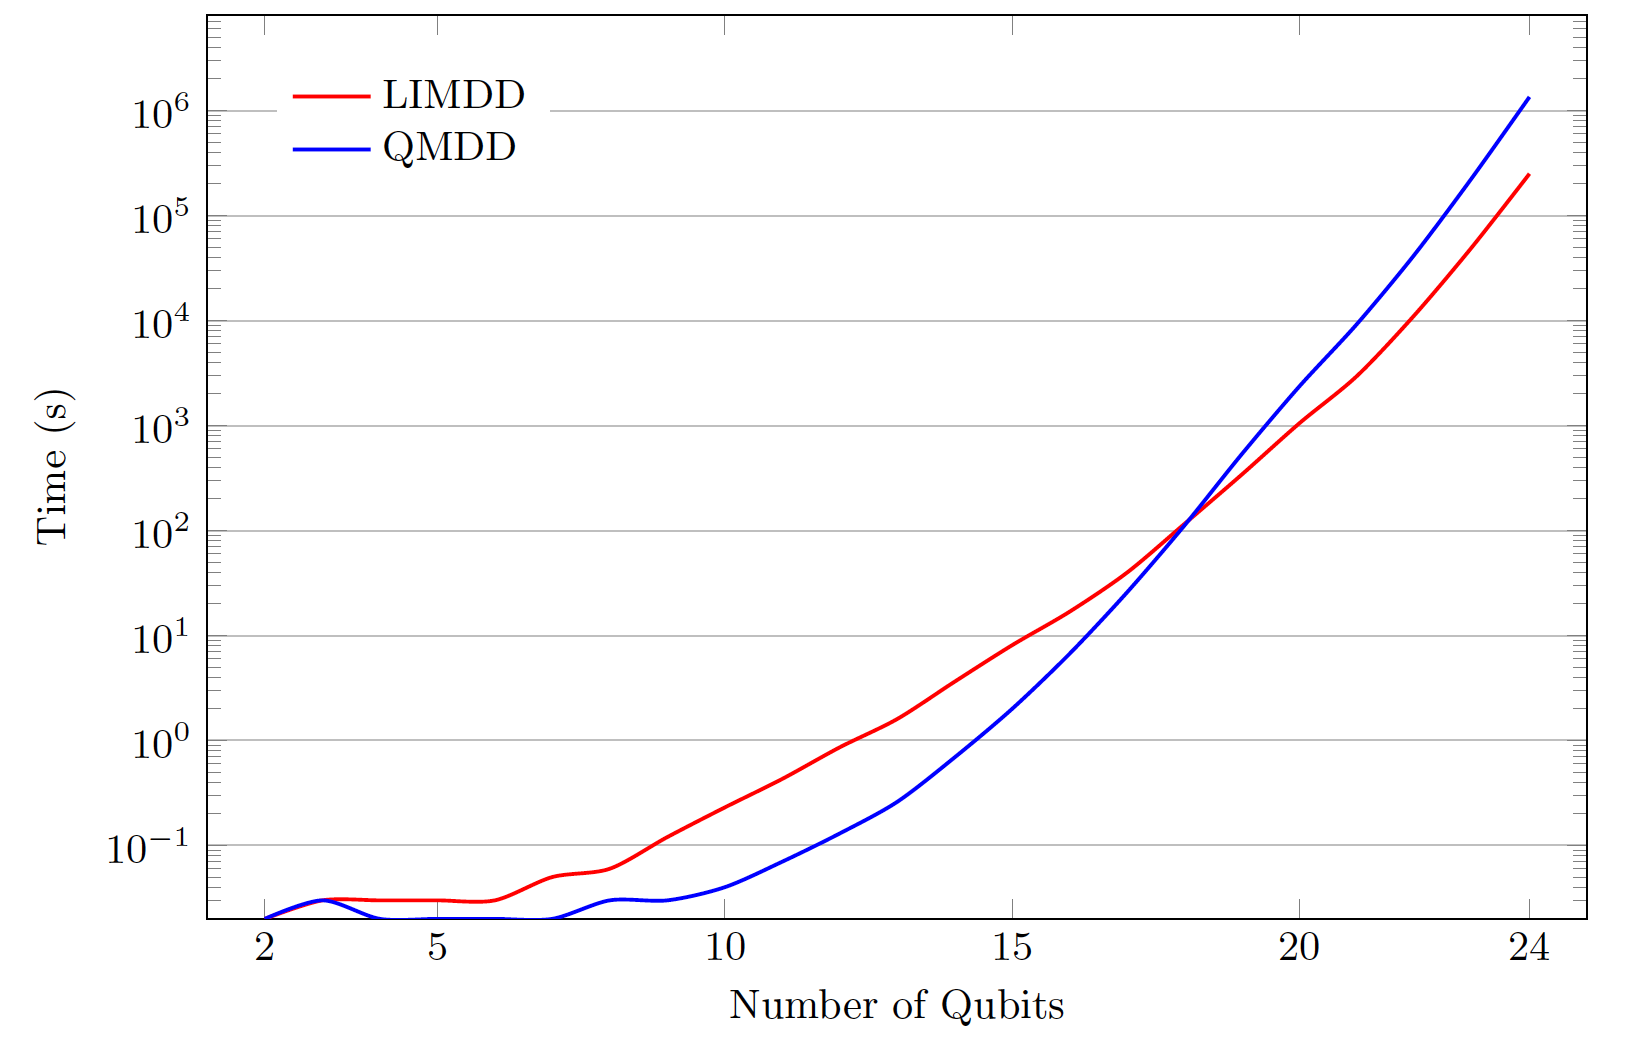
\includegraphics[height=5.cm]{plot.png}

\vspace{-.5em}

\centering
\printbibliography[section=\therefsection]
\vspace{-1em}
\url{https://github.com/cda-tum/mqt-limdd}


\end{frame}
\end{refsection}





%\begin{refframe}{Chronology of Decision Diagrams for Pseudo-Boolean Functions}
%	
%\vspace{-.8em}
%
%
%%\begin{table}
%%\centering\footnotesize
%%\def\arraystretch{1.1}
%%\begin{tabular}{|p{5.5cm}|c|c|}
%%\hline
%%\textbf{Decision diagrams for pseudo-Boolean functions}				& \textbf{Node merging strategy} &  \\\hline
%%%Decision Tree	& (no merging) &  \\
%%MTBDD~(1993)~\cite{clarke1993spectral}, \add~(1997)~\cite{bahar1997algebric}	& $f = g$  &  \\
%%SLDD$_\times$~(2005)~\cite{wilson2005decision}	& $f = \gamma\cdot g$   & $\gamma \in \complex, \mathbb R, \dots$  \\
%%EVBDD (1994)~\cite{lai1994evbdd}, SLDD$_+$ (2013)~\cite{fargier2013semiring}	& $f = g + \alpha$ & $\alpha \in \complex, \mathbb R, \dots$  \\
%%FEVBDD~(1997)~\cite{tafertshofer1997factored}, AADD~(2005)~\cite{sanner2005AffineADDs}		& $f = \gamma\cdot g + \alpha$ & $\alpha,\gamma \in \complex, \mathbb R, \dots$ \\
%%%\limdd~\cite{limdd}			& $f = \gamma  P_1\otimes \dots \otimes P_n \cdot g$ & $P_i \in \gen{\id, X,Y,Z}$   \\
%%\hline
%%\end{tabular}
%%\end{table}
%
%
%\begin{table}
%\centering\footnotesize
%\def\arraystretch{2}
%\begin{tabular}{|p{5cm}|c|c|}
%\hline
%\textbf{Quantum variant}				& \textbf{Node merging} &  \\\hline
%%Decision Tree	& (no merging) &  \\
% QuiDD~(2003)~\cite{viamontes2003improving}					    & $f = g$  &  \\
% QMDD~(2006)~\cite{miller2006qmdd}, TDD~(2020)~\cite{hong2020tensor}   & $f = \gamma\cdot g$   & $\gamma \in \complex$  \\
%%SLDD$_+$~\cite{fargier2013semiring}, EVBDD~\cite{lai1994evbdd}	& $f = g + \alpha$ & $\alpha \in \complex, \mathbb R, \dots$  \\
%%AADD~\cite{sanner2005AffineADDs}, FEVBDD~\cite{tafertshofer1997factored} 		& $f = \gamma\cdot g + \alpha$ & $\alpha,\gamma \in \complex, \mathbb R, \dots$ \\
%%QDD~(2008)~\cite{wang2008xqdd}					& $f =  R_X(\theta) \cdot g$  & $\theta \in \real$ \\
%\limdd~(2021)~\cite{limdd}			& $f = \gamma  P_1\otimes \dots \otimes P_n \cdot g$ & $P_i \in \gen{\id, X,Y,Z}$   \\
%CFLOBDD~(2023)~\cite{sistla2023weighted}				& (more like SDD)  & \\
%\hline
%\end{tabular}
%\end{table}
%
%\vspace{-.8em}
%
%
%\nocite{limdd2}
%
%\end{refframe}
%






